\hypertarget{mux1ee5c-tiuxeau-dux1ef1-uxe1n}{%
\section{Mục tiêu dự án}\label{mux1ee5c-tiuxeau-dux1ef1-uxe1n}}

Mục tiêu của dự án này là thực hiện hệ thống điểm danh sử dụng nhận diện
khuôn mặt phối hợp với thẻ RFID/NFC. Phần cứng được sử dụng sẽ là board
mạch Raspberry Pi 4 và viết hoàn toàn bằng Python 3.

Hệ thống này này sẽ có khả năng:

\begin{itemize}
\tightlist
\item
  Đọc thẻ từ người dùng
\item
  Sử dụng một cơ sở dữ liệu nhỏ để truy xuất các thông tin cần thiết cho
  việc nhận diện khuôn mặt
\item
  Sử dụng nhận diện khuôn mặt ứng với dữ liệu được lưu. Nếu hoàn tất,
  xác thực thành công. Ngược lại từ chối.
\item
  Có khả năng đăng kí khuôn mặt người dùng vào cơ sở dữ liệu
\end{itemize}

\hypertarget{muxe3-nguux1ed3n-vuxe0-cuxe1c-tuxe0i-liux1ec7u-cux1ee7a-dux1ef1-uxe1n}{%
\section{Mã nguồn và các tài liệu của dự
án}\label{muxe3-nguux1ed3n-vuxe0-cuxe1c-tuxe0i-liux1ec7u-cux1ee7a-dux1ef1-uxe1n}}

Tất cả mọi mã nguồn, bao gồm báo cáo này, slide thuyết trình, các ghi
chú trong việc tìm hiểu đều được lưu lại trên GitHub:
\url{https://github.com/ntpt7921/RaspPi_AttendanceSystem}

\hypertarget{phux1ea7n-cux1ee9ng-vuxe0-phux1ea7n-mux1ec1m-sux1eed-dux1ee5ng}{%
\section{Phần cứng và phần mềm sử
dụng}\label{phux1ea7n-cux1ee9ng-vuxe0-phux1ea7n-mux1ec1m-sux1eed-dux1ee5ng}}

\hypertarget{phux1ea7n-cux1ee9ng}{%
\subsection{Phần cứng}\label{phux1ea7n-cux1ee9ng}}

\begin{itemize}
\tightlist
\item
  Raspberry Pi 4 (2GB RAM) - yếu điểm của dự án
\item
  PN532 module
  (\href{https://hshop.vn/products/mach-rfid-nfc-13-56mhz-pn532}{Hshop})
\item
  Camera Raspberry Pi V1 OV5647
  (\href{https://hshop.vn/products/camera-raspberry-pi}{Hshop})
\item
  MIFARE Classic 1K
  (\href{https://hshop.vn/products/the-nhua-nfc-philips-s50rfid-13-56-mhz}{Hshop})
\end{itemize}

\hypertarget{phux1ea7n-mux1ec1m}{%
\subsection{Phần mềm}\label{phux1ea7n-mux1ec1m}}

\begin{itemize}
\tightlist
\item
  Thư viện thị giác máy tính OpenCV
  (\href{https://docs.opencv.org/4.5.1/}{documentation chính thức}),
  phiên bản 4.5.1
\item
  Thư viện cho module PN532 của Waveshare
  (\href{https://www.waveshare.com/wiki/PN532_NFC_HAT}{documentation
  chính thức}))
\end{itemize}

\hypertarget{kux1ebft-quux1ea3}{%
\section{Kết quả}\label{kux1ebft-quux1ea3}}

Thất bại trong việc ứng dụng hệ thống nhận diện khuôn mặt. Trong các mục
tiêu đã đề ra:

\begin{itemize}
\tightlist
\item
  Đọc thẻ từ người dùngt

  \begin{itemize}
  \tightlist
  \item
    Có khả năng đọc thẻ từ người dùng, đã thử thành công trên phần cứng
  \end{itemize}
\item
  Sử dụng một cơ sở dữ liệu nhỏ

  \begin{itemize}
  \tightlist
  \item
    Có ứng dụng một cơ sở dữ liệu dùng để map ID của thẻ thành tên mô
    hình để nhận diện khuôn mặt, đã thử thành công trên phần cứng
  \end{itemize}
\item
  Sử dụng nhận diện khuôn mặt

  \begin{itemize}
  \tightlist
  \item
    Đã thử nghiệm trên máy laptop cá nhân và chạy được. Không thể khởi
    động camera của Raspberry Pi để có thể thử. Không thể phân biệt được
    khuôn mặt thật và bức ảnh của khuôn mặt
  \end{itemize}
\item
  Có khả năng đăng kí khuôn mặt mới

  \begin{itemize}
  \tightlist
  \item
    Cũng đã thử nghiệm trên máy laptop và chạy được. Không dùng camera
    trên Raspberry Pi được
  \end{itemize}
\end{itemize}

Thất bại trong mục tiêu chính, nội dung chính của báo cáo này là miêu tả
các phần đã làm được và nhìn nhận về lí do thât bại.

\hypertarget{cux1ea5u-truxfac-chung-cho-touxe0n-dux1ef1-uxe1n}{%
\section{Cấu trúc chung cho toàn dự
án}\label{cux1ea5u-truxfac-chung-cho-touxe0n-dux1ef1-uxe1n}}

Phân tích công việc cần phải thực hiện ta có thể chia dự án này ra làm
các phần

\begin{itemize}
\tightlist
\item
  \protect\hyperlink{RFID_NFC}{RFID/NFC}: Tìm hiểu cách đẻ đọc được thẻ
  + các thông tin liên quan
\item
  \protect\hyperlink{Database}{Database}: Tìm hiểu cách để có thể lưu và
  truy xuất dữ liệu của nhiều cá nhân
\item
  \protect\hyperlink{Face_Recog}{Face Recognition}: Tìm hiểu và ứng dụng
  việc nhận diện và phân biệt khuôn mặt người
\end{itemize}

Quy trình hoạt đông cơ bản của hệ thống được dự tính như sau: Hệ thống
sẽ liên tục dò các thẻ lân cận với bộ đọc. Trong trường hơp có một thẻ
(được cho ở đây)

\hypertarget{RFID_NFC}{%
\subsection{RFID/NFC}\label{RFID_NFC}}

Sử dụng module PN532 và thư viện PN532 NFC HAT của Waveshare, việc đọc
thẻ có thể được thực hiện khá dễ dàng.

\begin{figure}
\centering
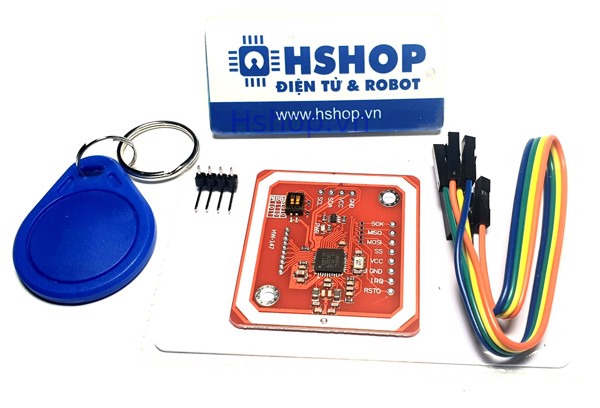
\includegraphics{PN532_module.jpeg}
\caption{Hình của module PN532. Lấy từ trang của Hshop}
\end{figure}

Sử dụng chip PN532, ta có khả năng đọc và ghi thẻ Mifare 1K. Trong dự án
này ta sẽ sử dụng hai chức năng được thư viện cung cấp: đợi thẻ, và đọc
thẻ.

Có thể thấy rằng thư viện mà Waveshare cung cấp cho board mà họ sản xuất
không thực sự giống với module mua được từ Hshop. Việc sử dụng thư viện
này là vì trong bước đàu tim hiểu, không tìm thấy thư viện Python cho
board mua được. Nên việc chọn thư viện phụ thuộc chủ yếu vào việc so
sánh các board được chung cấp chính thức sử dụng thư viện và board mua,
rồi đọc qua thư viện để xem xét liệu có thể thay thế module hay không.
Sau khi coi qua thư viện của Adafruit, và Seeed Studio và Waveshare,
Waveshare được chọn.

Về phần cứng, phải hàn thêm một số đường tín hiệu, sao chép cho đúng với
board breakout chính thức.

Sau khi tìm hiểu thêm, một thư viện khác tương thích hơn nhiều trên
\href{https://pypi.org/project/pn532pi/}{PyPi} được tìm thấy. Nhưng đã
viết quá nhiều mã phụ thuộc và thời gian không cho phép, nên không thể
thay thế thư viện được.

Lợi dụng tính chất sẵn có của thẻ Mifare - block đầu tiên (số 0) của
sector 0 là chỉ đọc và sẽ là nơi lưu trữ UID (unique ID) của thẻ và các
thông tin của nhà sản xuất, ta có thể sử dụng nội dung block này để định
danh thẻ mà không cần phải thực hiện ghi vào các block còn lại. Điều này
nghĩa là ta sẽ có 16 byte dữ liệu (độ lớn block) để định danh thẻ.

Thông tin thêm về RFID/NFC được lưu trong file
\href{https://github.com/ntpt7921/RaspPi_AttendanceSystem/blob/main/nfc/NOTE.md}{\texttt{NOTE.md}},
nằm trong thư mục
\href{https://github.com/ntpt7921/RaspPi_AttendanceSystem/tree/main/nfc}{\texttt{nfc}}.

\hypertarget{Database}{%
\subsection{Database}\label{Database}}

Thành phần thứ hai phục vụ chức năng của dự án. Kém quan trọng hơn hai
thành phần kia nếu không xét tới tính bảo mật của hệ thống (bảo mật
không phải điểm tập trung của dự án).

Mục tiêu ban đầu của thành phần này là thực hiện một cơ sở dữ liệu nhỏ
được lưu trên mạng, vơi sao chép dữ liệu được lưu cục bộ trong Raspberry
Pi, dữ liệu lưu trữ dạng chữ.

Giới hạn thời gian chỉ cho phép thực hiện một bộ nhớ cơ bản (sử dụng cấu
trúc \texttt{dict} của Python). Bộ lưu dữ liệu này sẽ thực hiện việc map
một key nào đó (ở đây là sẽ là số định danh thẻ được chuyển từ 16 byte
thành số nguyên) sang phần data (tên của model phân biệt khuôn mặt ứng
với người dùng của thẻ). Bộ nhớ này có thể lưu thông tin của nó và một
file JSON và nạp từ file JSON này để lưu trữ lâu dài. Việc lưu trữ file
JSON này sẽ được thực hiện trên phần cứng cục bộ (thẻ nhớ của Raspberry
Pi).

\begin{Shaded}
\begin{Highlighting}[]
\FunctionTok{\{}
    \DataTypeTok{"1"}\FunctionTok{:} \StringTok{"YuqJrMLmWKZJIkj88qFQSlHWLH5gg7"}\FunctionTok{,}
    \DataTypeTok{"2"}\FunctionTok{:} \StringTok{"zDSi7Bv8LE9Y63yVZT0AIyUpsNBaGB"}\FunctionTok{,}
    \DataTypeTok{"3"}\FunctionTok{:} \StringTok{"TNXr6jYbokuuM0yPJr2GqesRUDRGzk"}
\FunctionTok{\}}
\end{Highlighting}
\end{Shaded}

\hypertarget{Face_Recog}{%
\subsection{Face Recognition}\label{Face_Recog}}

Ta sử dụng thư viện OpenCV đê thực hiện dự án này. Cụm từ `nhận diện
khuôn mặt' tới bây giờ chỉ chung việc trích tách hình ảnh khuôn mặt và
phân biệt khuôn mặt từ một tập các khuôn mặt đã biết. Chức năng này bao
hàm hai thành phần lớn bao mà ta phân biệt và hiện thực riêng trong dự
án này: - Phát hiện và trích tách khuôn mặt (Face detection): Dò hình
ảnh được cho và chỉ ra vị trí mà khuôn mặt người xuất hiện trong hình. -
Nhận biết khuôn mặt (Face recognition): Lấy hình ảnh một khuôn mặt và
xem xét liệu khuôn mặt được cho có là một trong nhưng khuôn mặt đã biết
trước, và nếu có thì xác định chính xác khuôn mặt nào.

Ta tập trung vào ứng dụng thư viện cung cấp khả năng nhận cân thiết, chứ
không chú trọng vào thí thuyết hoạt động.

\hypertarget{phuxe1t-hiux1ec7n-vuxe0-truxedch-xuux1ea5t}{%
\subsubsection{Phát hiện và trích
xuất}\label{phuxe1t-hiux1ec7n-vuxe0-truxedch-xuux1ea5t}}

Thư viện OpenCV cung cấp nhiều phương pháp để có thể phát hiện khuôn
mặt:

\begin{itemize}
\tightlist
\item
  LBP Cascade
\item
  Haar Cascade
\item
  DNN
\end{itemize}

So sánh các phương pháp, LBP là nhanh nhất, nhưng kém chính xác. Haar
chậm hơn nhưng lại chính xác hơn. DNN có thể hoạt động nhanh bằng Haar
với độ chính xác rất tốt. Các kết luận so sánh này được tổng hợp từ các
bài viết tham khảo của mục này.

Trong dự án này ta mặc định sử dụng DNN, nhưng phưowng pháp phát hiện có
thể được thay đổi khi khởi tạo các hàm liên quan. k \#\#\# Nhận biết
khuôn mặt

Cũng tồn tại nhiều phương pháp để nhận biết khuôn mặt, được cung cấp bởi
nhiều thư viện khác nhau. Nhưng trong khuôn khổ dự án nầy ta chỉ dùng
LBPH của OpenCV. Phương thức hoạt động của LBHP cũng gần giống với LBP,
và là một phương pháp khá dễ hiểu và nguyên tắc.

Không có lí do đặc biệt gì để chọn sử dụng phương pháp này ngoài việc
đây là một trong nhũng phương pháp đầu tiên tìm được khi tìm hiểu. Sau
khi viết mã và kiểm thử, vì không phát hiện ra điểm gì không thích hơn
nên cũng không ứng dụng thêm các phương pháp khác.

Một số bài viết tham khảo được ghi chú lại trong file
\href{https://github.com/ntpt7921/RaspPi_AttendanceSystem/blob/main/face_recognition/NOTE.md}{\texttt{NOTE.md}}
trong thư mục
\href{https://github.com/ntpt7921/RaspPi_AttendanceSystem/tree/main/face_recognition}{\texttt{face\_regconition}}

\hypertarget{vux1ea5n-ux111ux1ec1}{%
\section{Vấn đề}\label{vux1ea5n-ux111ux1ec1}}

Vấn đề lớn nhất chưa giải quyết được của dự án này là việc thư viện
OpenCV không thể khởi động được camera trên Raspberry Pi.

\begin{figure}
\centering
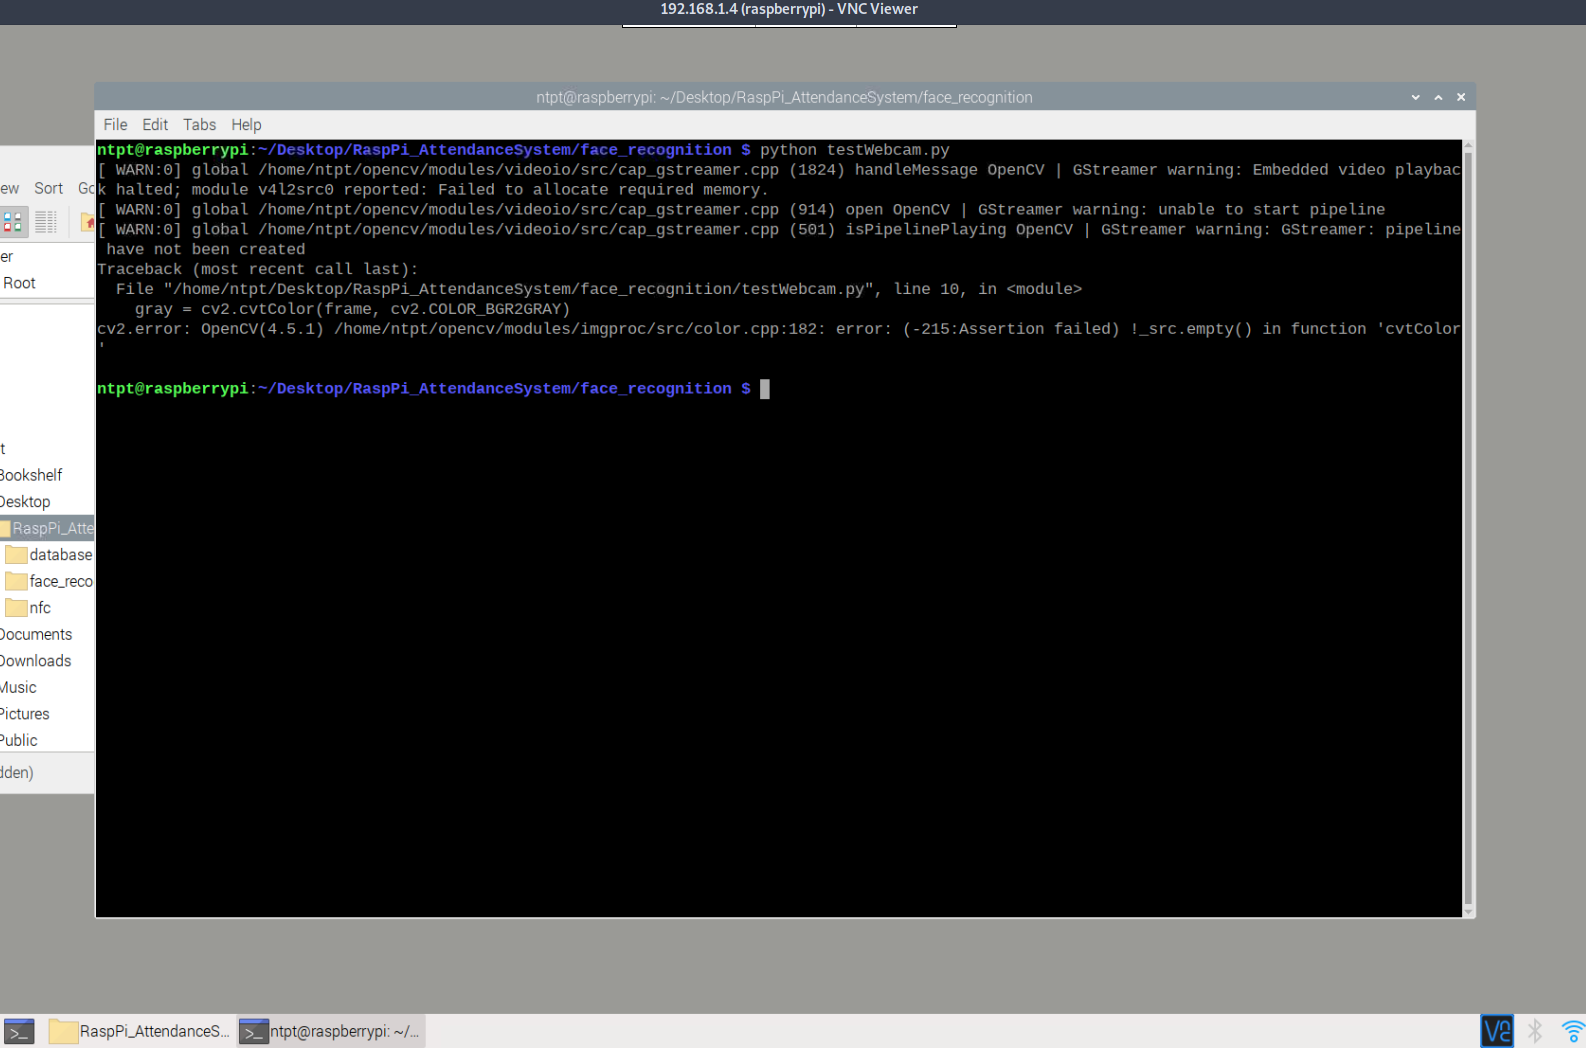
\includegraphics{raspi_camera_error.png}
\caption{Lôi khi khổi động camera trên Raspberry Pi}
\end{figure}

Tìm hiểu và thử nghiệm qua nhiêu cách khác nhau (cài lai thư viện bằng
nguồn khác, compile lại thư viện), lỗi này vẫn không giải quyết được.
Cần thêm nhiều thời gian để tìm hiểu lý do. NHưng hiện giờ lời giải
thích tốt nhất là Raspberry không có đủ bộ nhớ RAM để khởi động camera.

\hypertarget{nhuxecn-nhux1eadn}{%
\section{Nhìn nhận}\label{nhuxecn-nhux1eadn}}

Có thể phân ra một số lí do cho thất bại lần này, nhiều điểm không thể
tránh khỏi

\begin{itemize}
\tightlist
\item
  Thiếu hiểu biết về Raspberry Pi
\item
  Thiếu kinh nghiệm về ngôn ngữ Python
\item
  Chọn đề tài quá khó để có thể thực hiện
\end{itemize}

\hypertarget{tuxe0i-liux1ec7u-tham-khux1ea3o}{%
\section{Tài liệu tham khảo}\label{tuxe0i-liux1ec7u-tham-khux1ea3o}}

Phân tán rải rác và có rất nhiều, tham khảo

\begin{itemize}
\tightlist
\item
  \href{https://github.com/ntpt7921/RaspPi_AttendanceSystem/blob/main/face_recognition/NOTE.md}{Note
  của phần nhận diện mặt}
\item
  \href{https://github.com/ntpt7921/RaspPi_AttendanceSystem/blob/main/nfc/NOTE.md}{Note
  của phần RFID/NFC}
\end{itemize}
